%% ========================================================================
%% Chapter 10: Memory Management & System Calls
%% ========================================================================
\chapter{Memory Management \& System Calls}
\label{ch:memory-and-syscalls}

Imagine your desk. Documents you are actively working on sit on the desk surface
--- this is analogous to \textbf{RAM}. When the desk gets full, some documents
are moved to a drawer to make room --- this is analogous to \textbf{swap}. If
all documents end up in the drawer and you keep going back and forth to retrieve
them, work slows to a crawl. That is a simple picture of how Linux manages memory.

In this chapter we will explore that concept in depth, and also learn about
\textbf{system calls} --- the mechanism programs use to request services from the
kernel. We will also put the Bash skills from Chapter~9 to work building real,
useful monitoring scripts.

\textbf{Lab Objectives}

After completing this lab, students should be able to:

\begin{enumerate}
    \item understand the memory architecture on Linux;
    \item explain the concept of virtual memory and the paging mechanism;
    \item manage and configure swap space;
    \item monitor memory usage using various tools;
    \item understand the concept and types of system calls;
    \item observe the interaction between user space and kernel space.
\end{enumerate}

\begin{notebox}
All lab tasks are run as a regular user unless the command explicitly uses
\texttt{sudo}. Create the working directory first:
\begin{lstlisting}
mkdir -p ~/lab-os/week10-memory
\end{lstlisting}
\end{notebox}

\section{Memory Architecture on Linux}

\textbf{Concept Overview}

Every program running on Linux gets its own \textit{virtual address space}.
This means each program behaves as if it has private memory that cannot be
touched by other programs. The kernel is responsible for mapping those virtual
addresses to physical memory (RAM).

The virtual address space of a process is divided into several areas with
distinct roles, as shown in \cref{fig:memory-layout}.

\begin{figure}[H]
\centering
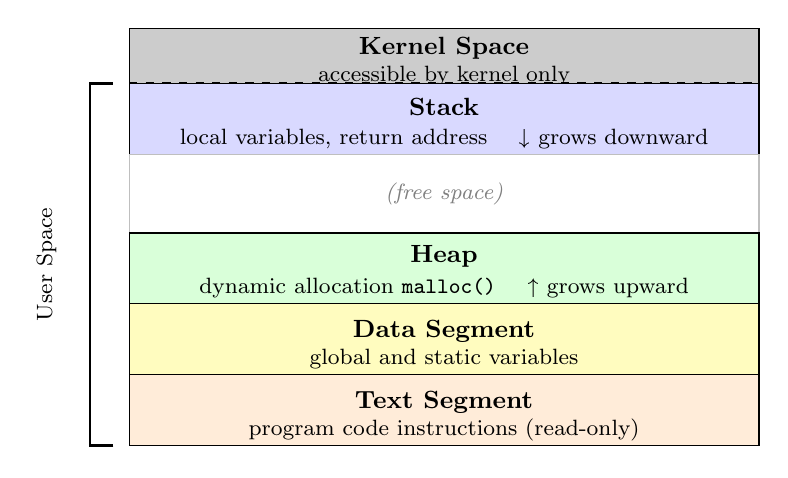
\begin{tikzpicture}[font=\small]
    % Kernel Space
    \filldraw[fill=gray!40, draw=black] (0,5.0) rectangle (8,5.7);
    \node[font=\small\bfseries] at (4, 5.45) {Kernel Space};
    \node[font=\footnotesize] at (4, 5.1) {accessible by kernel only};
    % Boundary
    \draw[dashed, thick] (0,5.0) -- (8,5.0);
    % Stack
    \filldraw[fill=blue!15, draw=black] (0,4.1) rectangle (8,5.0);
    \node[font=\small\bfseries] at (4, 4.7) {Stack};
    \node[font=\footnotesize] at (4, 4.3) {local variables, return address \quad ↓ grows downward};
    % Free space
    \draw[draw=gray!50] (0,3.1) rectangle (8,4.1);
    \node[font=\footnotesize\itshape, gray] at (4, 3.6) {(free space)};
    % Heap
    \filldraw[fill=green!15, draw=black] (0,2.2) rectangle (8,3.1);
    \node[font=\small\bfseries] at (4, 2.8) {Heap};
    \node[font=\footnotesize] at (4, 2.4) {dynamic allocation \texttt{malloc()} \quad ↑ grows upward};
    % Data
    \filldraw[fill=yellow!25, draw=black] (0,1.3) rectangle (8,2.2);
    \node[font=\small\bfseries] at (4, 1.85) {Data Segment};
    \node[font=\footnotesize] at (4, 1.5) {global and static variables};
    % Text
    \filldraw[fill=orange!15, draw=black] (0,0.4) rectangle (8,1.3);
    \node[font=\small\bfseries] at (4, 0.95) {Text Segment};
    \node[font=\footnotesize] at (4, 0.6) {program code instructions (read-only)};
    % User Space bracket (left side, inside figure bounds)
    \draw[thick] (-0.2,0.4) -- (-0.5,0.4) -- (-0.5,5.0) -- (-0.2,5.0);
    \node[font=\footnotesize, rotate=90, anchor=south] at (-0.8, 2.7) {User Space};
\end{tikzpicture}
\caption{Virtual memory map of a Linux process. Each process has its own isolated
virtual address space, separate from all other processes.}
\label{fig:memory-layout}
\end{figure}

\begin{notebox}
Process isolation guarantees system stability. If one program crashes, the damage
is contained to that process --- other processes continue running normally because
they cannot access each other's memory.
\end{notebox}

\textbf{Commands Used}

\begin{itemize}
    \item \texttt{free -h}: summary of RAM and swap usage in human-readable format.
    \item \texttt{cat /proc/meminfo}: detailed memory information directly from the kernel.
    \item \texttt{top}: monitor system resource usage in real time.
\end{itemize}

\subsection*{Lab 10.1 Viewing Memory Usage}

\textbf{Objective}: identify the structure and usage of memory on a Linux system.

\textbf{Step 1}: Run \texttt{free -h} to see a summary of RAM and swap.

\begin{lstlisting}[caption={Viewing memory usage}]
free -h
\end{lstlisting}

The output of \texttt{free -h} shows two rows: \texttt{Mem} for RAM and
\texttt{Swap} for swap. Key columns in the \texttt{Mem} row:
\begin{itemize}
    \item \texttt{total}: total installed RAM.
    \item \texttt{used}: memory currently used by processes and the kernel.
    \item \texttt{free}: memory that is completely unused, not allocated at all.
    \item \texttt{available}: estimated memory \textit{truly available} to new
    applications, including reclaimable cache. Use this value, not \texttt{free},
    to assess the system's memory health.
    \item \texttt{buff/cache}: memory used by the kernel as I/O buffers and file
    cache. Linux reclaims this cache automatically whenever an application needs it.
\end{itemize}

\textbf{Step 2}: View detailed memory information from the kernel via \texttt{/proc/meminfo}.

\begin{lstlisting}[caption={Viewing kernel memory details}]
cat /proc/meminfo | head -n 20
\end{lstlisting}

\textbf{Analysis:}

\begin{enumerate}
    \item Calculate the percentage of available memory: \texttt{available / total × 100\%}.
    If the result is below 10\%, the system is starting to run low on memory.
    \item On the \texttt{Swap} row, is the \texttt{used} column equal to 0? If it
    is greater than 0, the kernel has already moved data to disk because RAM was
    insufficient.
    \item Note the \texttt{Cached} and \texttt{Buffers} fields in \texttt{/proc/meminfo}.
    These values correspond to the \texttt{buff/cache} column in \texttt{free -h}.
\end{enumerate}

\begin{tipbox}
Do not worry if the \texttt{used} value appears large. Linux intentionally uses
idle RAM as a file cache to speed up disk access. Focus on \texttt{available}
--- that is the memory truly available for applications.
\end{tipbox}

\subsection*{Case Study 10.1 Server Slow Due to Memory}

\textbf{Scenario}: An application server feels slow when many users are active.
The administrator needs to determine whether the cause is insufficient memory.

\textbf{Step 1}: Check the overall memory condition.

\begin{lstlisting}[caption={Initial memory condition check}]
free -h
\end{lstlisting}

\textbf{Step 2}: Monitor processes in real time.

\begin{lstlisting}[caption={Real-time monitoring with top}]
top
\end{lstlisting}

Inside \texttt{top}: press \keystroke{M} to sort by memory, press
\keystroke{q} to quit.

\textbf{Analysis:}

\begin{enumerate}
    \item Is the \texttt{available} value very small (for example below 200~MB on
    a server with 2~GB RAM)? If so, the server is likely running out of memory.
    \item Is the \texttt{used} column on the \texttt{Swap} row greater than 0? If
    yes, the kernel is using swap, meaning performance has degraded.
    \item In the \texttt{top} display, which process has the highest \texttt{\%MEM}?
    That process is the primary candidate causing the server's slowness.
\end{enumerate}

\section{Virtual Memory Management}

\textbf{Concept Overview}

Imagine a large library with thousands of books. You can only place a few books
on your reading table (RAM), while the rest stay on the shelves (disk/swap).
When you need a book from the shelf, you must fetch it and perhaps return another
book to make room. That is how \textit{virtual memory} and \textit{paging} work.

Virtual memory allows programs to use more memory than the available RAM.
Data is divided into fixed-size blocks called \textbf{pages}. The kernel
automatically moves inactive pages to swap (\textit{swap out}) and loads them
back when needed (\textit{swap in}), as illustrated in \cref{fig:virtual-memory}.

\begin{figure}[H]
\centering
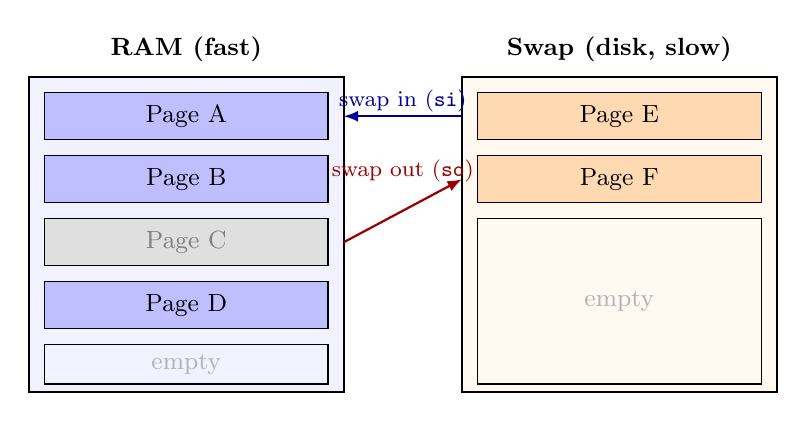
\begin{tikzpicture}[font=\small, >=latex]
    % RAM box (0..4 x 0..4)
    \draw[fill=blue!5, thick] (0,0) rectangle (4,4);
    \node[font=\small\bfseries] at (2, 4.35) {RAM (fast)};
    \filldraw[fill=blue!25]  (0.2,3.2) rectangle (3.8,3.8); \node at (2,3.5) {Page A};
    \filldraw[fill=blue!25]  (0.2,2.4) rectangle (3.8,3.0); \node at (2,2.7) {Page B};
    \filldraw[fill=gray!25]  (0.2,1.6) rectangle (3.8,2.2); \node[gray] at (2,1.9) {Page C};
    \filldraw[fill=blue!25]  (0.2,0.8) rectangle (3.8,1.4); \node at (2,1.1) {Page D};
    \draw (0.2,0.1) rectangle (3.8,0.6); \node[gray!60] at (2,0.35) {empty};
    % Swap box (5.5..9.5 x 0..4)
    \draw[fill=orange!5, thick] (5.5,0) rectangle (9.5,4);
    \node[font=\small\bfseries] at (7.5, 4.35) {Swap (disk, slow)};
    \filldraw[fill=orange!30] (5.7,3.2) rectangle (9.3,3.8); \node at (7.5,3.5) {Page E};
    \filldraw[fill=orange!30] (5.7,2.4) rectangle (9.3,3.0); \node at (7.5,2.7) {Page F};
    \draw (5.7,0.1) rectangle (9.3,2.2); \node[gray!60] at (7.5,1.15) {empty};
    % Arrows (between boxes, labels inside the gap)
    \draw[->, thick, red!60!black] (4,1.9) -- (5.5,2.7);
    \node[font=\footnotesize, red!60!black] at (4.75, 2.8) {swap out (\texttt{so})};
    \draw[->, thick, blue!60!black] (5.5,3.5) -- (4,3.5);
    \node[font=\footnotesize, blue!60!black] at (4.75, 3.7) {swap in (\texttt{si})};
\end{tikzpicture}
\caption{Paging mechanism: the kernel moves inactive pages to swap when RAM is full,
and loads them back (\texttt{si}/\texttt{so} in \texttt{vmstat}) when needed.}
\label{fig:virtual-memory}
\end{figure}

\textbf{Commands Used}

\begin{itemize}
    \item \texttt{vmstat 1 5}: virtual memory, CPU, and I/O statistics every 1 second
    for 5 samples. The \texttt{si} (swap in) and \texttt{so} (swap out) columns are
    the primary indicators of paging activity.
\end{itemize}

\subsection*{Lab 10.2 Observing Paging Activity}

\textbf{Objective}: understand virtual memory activity through the swap columns in \texttt{vmstat}.

\textbf{Step 1}: Run \texttt{vmstat} with a 1-second interval, 5 samples.

\begin{lstlisting}[caption={Viewing virtual memory statistics}]
vmstat 1 5
\end{lstlisting}

In the output, locate the \texttt{swap} section containing two sub-columns:
\begin{itemize}
    \item \texttt{si}: KB/second moved from disk to RAM. A value of 0 means no
    data is currently being loaded from swap.
    \item \texttt{so}: KB/second moved from RAM to disk. A value of 0 means RAM
    is still sufficient and no data is being pushed to swap.
\end{itemize}

\textbf{Analysis:}

\begin{enumerate}
    \item Observe the \texttt{si} and \texttt{so} values across all five rows. On
    a system with adequate RAM, both values should always be 0.
    \item If \texttt{si} or \texttt{so} occasionally shows a value greater than 0,
    some swap activity has occurred. This is still acceptable if it is not continuous.
    \item If \texttt{si} and \texttt{so} are consistently greater than 0, the system
    is under serious \textit{memory pressure} --- performance drops sharply because
    disk access is far slower than RAM.
    \item Also observe the \texttt{free} (available RAM) and \texttt{buff} (buffers)
    columns to understand the overall RAM condition at that moment.
\end{enumerate}

\begin{warningbox}
Persistently high \texttt{si} and \texttt{so} values indicate the system needs
more RAM. Solutions: add RAM, reduce the number of concurrent processes, or
optimize application configuration.
\end{warningbox}

\section{Swap Space Configuration}

\textbf{Concept Overview}

Swap space is an area on disk that acts as an extension of RAM. Swap prevents
the system from crashing when RAM is exhausted, but because it resides on disk,
access is far slower. Swap is a \textit{safety net}, not a replacement for RAM.

The \texttt{swappiness} parameter (values 0--100) controls how aggressively the
kernel uses swap:
\begin{itemize}
    \item \textbf{High value (60--100)}: the kernel quickly moves data to swap
    even when RAM is still available. This is the Linux default (60).
    \item \textbf{Low value (10--20)}: the kernel prefers to keep data in RAM
    and only uses swap when truly necessary. Recommended for application servers.
\end{itemize}

\textbf{Commands Used}

\begin{itemize}
    \item \texttt{swapon --show}: list active swap areas with their size and usage.
    \item \texttt{fallocate -l \textit{size} \textit{file}}: efficiently create an
    empty file of a specified size.
    \item \texttt{mkswap \textit{file}}: format a file as a swap area.
    \item \texttt{swapon}/\texttt{swapoff}: activate/deactivate swap.
    \item \texttt{sysctl vm.swappiness=\textit{value}}: temporarily change swappiness.
\end{itemize}

\subsection*{Lab 10.3 Creating and Configuring a Swap File}

\textbf{Objective}: add swap space and understand the swappiness parameter.

\textbf{Step 1}: Create a 512~MB file to use as swap.

\begin{lstlisting}[caption={Creating a 512MB swap file}]
sudo fallocate -l 512M /swapfile-week10
\end{lstlisting}

\textbf{Step 2}: Set the file permission to \texttt{600} --- only root may read
and write it.

\begin{lstlisting}[caption={Securing swap file permissions}]
sudo chmod 600 /swapfile-week10
\end{lstlisting}

\begin{warningbox}
This step is \textbf{mandatory} before running \texttt{mkswap}. A swap file can
contain fragments of sensitive data from program memory. Open permissions
(\texttt{644}) would allow other users to read the contents of that memory.
\end{warningbox}

\textbf{Step 3}: Format the file as a swap area, then activate it.

\begin{lstlisting}[caption={Formatting and activating swap}]
sudo mkswap /swapfile-week10
sudo swapon /swapfile-week10
\end{lstlisting}

\textbf{Step 4}: Verify the swap is active. You should see the
\texttt{/swapfile-week10} entry with a size of 512M, and the \texttt{total} value
on the \texttt{Swap} row in \texttt{free -h} should increase by 512M.

\begin{lstlisting}[caption={Verifying swap is active}]
swapon --show
free -h
\end{lstlisting}

\textbf{Step 5}: Check the current swappiness value, temporarily change it, and
verify the change.

\begin{lstlisting}[caption={Viewing and changing swappiness}]
cat /proc/sys/vm/swappiness
sudo sysctl vm.swappiness=10
cat /proc/sys/vm/swappiness
\end{lstlisting}

\textbf{Analysis:}

\begin{enumerate}
    \item What is the default swappiness value? What does it mean for how aggressively
    the kernel uses swap?
    \item After changing to 10, confirm the value changed in the second \texttt{cat}
    output. What is the effect of a value of 10 on swap usage compared to 60?
    \item Does the \texttt{/swapfile-week10} entry appear in \texttt{swapon --show}?
    If not, ensure Step~2 (chmod 600) was run before Step~3.
\end{enumerate}

\begin{notebox}
Changes made via \texttt{sysctl} are temporary and lost after a reboot. For a
permanent setting, add \texttt{vm.swappiness=10} to \texttt{/etc/sysctl.conf}.

Clean up the swap file after the lab:
\begin{lstlisting}
sudo swapoff /swapfile-week10
sudo rm /swapfile-week10
\end{lstlisting}
\end{notebox}

\section{Memory Usage Monitoring}

\textbf{Concept Overview}

Memory monitoring helps administrators detect problems before they affect users.
There are two approaches:
\begin{itemize}
    \item \textbf{Real-time} with \texttt{top}: observe dynamic changes as they
    happen.
    \item \textbf{Snapshot} with \texttt{ps aux}: capture the process list at a
    single point in time, suitable for saving to a report file.
\end{itemize}

Key columns in \texttt{ps aux} output:
\begin{itemize}
    \item \texttt{\%MEM}: percentage of total RAM used by the process.
    \item \texttt{RSS} (Resident Set Size): physical RAM \textit{actually in use}
    by the process right now (in KB).
    \item \texttt{VSZ} (Virtual Memory Size): total virtual memory allocated,
    including portions not yet loaded into RAM (always larger than RSS).
\end{itemize}

\subsection*{Lab 10.4 Memory Monitoring}

\textbf{Objective}: identify the processes with the highest memory usage.

\textbf{Step 1}: Take a process snapshot sorted by highest memory usage.

\begin{lstlisting}[caption={Processes with the highest memory usage}]
ps aux --sort=-%mem | head
\end{lstlisting}

The first line is the header (column names). The process on the second line is
the largest memory consumer at the time the command was run.

\textbf{Step 2}: Monitor in real time with \texttt{top}.

\begin{lstlisting}[caption={Real-time monitoring}]
top
\end{lstlisting}

Inside \texttt{top}: \keystroke{M} = sort by memory,
\keystroke{P} = sort by CPU, \keystroke{q} = quit.

\textbf{Analysis:}

\begin{enumerate}
    \item Which process is at the top? Record its \texttt{\%MEM} and \texttt{RSS} values.
    \item Convert \texttt{RSS} from KB to MB (divide by 1024). For example,
    \texttt{RSS=524288} means the process is using 512~MB of RAM. Is that
    reasonable for that type of program?
    \item Why is \texttt{VSZ} always larger than \texttt{RSS} for the same process?
    \item Is the process order in \texttt{ps} consistent with \texttt{top} when
    sorted by \texttt{\%MEM}?
\end{enumerate}

\begin{tipbox}
Combine three tools: \texttt{free} for the global picture, \texttt{top} for
real-time dynamics, and \texttt{ps} for snapshots that can be saved to a file.
\end{tipbox}

\subsection*{Lab 10.5 Memory Monitor Script}

\textbf{Objective}: automate memory monitoring using a Bash script.

\begin{notebox}
This script applies concepts from Chapter~9: variables (\texttt{THRESHOLD}),
\texttt{if} conditionals, output parsing with \texttt{awk}, and the \texttt{date}
command to record the monitoring timestamp.
\end{notebox}

Navigate to the working directory and create the script file:

\begin{lstlisting}[caption={Navigate to directory and open nano}]
cd ~/lab-os/week10-memory
nano monitor-memory.sh
\end{lstlisting}

Type the following script:

\begin{lstlisting}[caption={Contents of monitor-memory.sh}]
#!/bin/bash
set -euo pipefail

THRESHOLD=20

echo "=== Memory Monitor ==="
date
echo

free -h
echo

AVAIL=$(free | awk '/Mem/ {printf "%d", $7/$2*100}')
if [ "$AVAIL" -lt "$THRESHOLD" ]; then
    echo "WARNING: Available memory is only ${AVAIL}%!"
else
    echo "Status: Available memory ${AVAIL}% (normal)"
fi
echo

echo "--- Top 5 Memory Processes ---"
ps aux --sort=-%mem | head -n 6 | tail -n 5
\end{lstlisting}

\begin{notebox}
Save: \keystroke{Ctrl+O} $\to$ \keystroke{Enter} $\to$ exit: \keystroke{Ctrl+X}.
\end{notebox}

\begin{lstlisting}[caption={Running the monitor script}]
chmod +x monitor-memory.sh
bash monitor-memory.sh
\end{lstlisting}

\textbf{Analysis:}

\begin{enumerate}
    \item The variable \texttt{THRESHOLD=20} sets the percentage threshold. The
    command \texttt{free | awk '/Mem/ \{printf "\%d", \$7/\$2*100\}'} reads column 7
    (available) divided by column 2 (total) from the \texttt{Mem} row, multiplied
    by 100 to produce an integer percentage.
    \item The condition \texttt{if [ "\$AVAIL" -lt "\$THRESHOLD" ]} is true when
    the available memory percentage is below 20.
    \item Change \texttt{THRESHOLD} to \texttt{90} and run again. What changes in
    the output? Why?
\end{enumerate}

\section{System Calls and User-Kernel Interaction}

\textbf{Concept Overview}

Imagine a restaurant. You (the program) cannot walk directly into the kitchen
(the kernel) to cook your own food --- you must order through a waiter (the
system call). The waiter relays your order to the kitchen, ensures it is valid,
and brings the result back to your table.

That is how a system call works: a mechanism for programs in \textit{user space}
to request services from the kernel. A program cannot directly access hardware,
the filesystem, or kernel resources --- all requests must go through system calls.
The complete flow is shown in \cref{fig:syscall-flow}.

\begin{figure}[H]
\centering
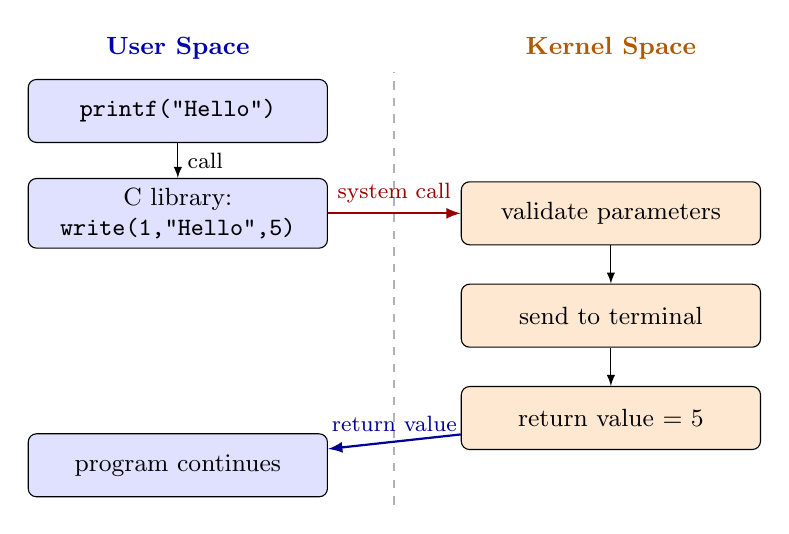
\begin{tikzpicture}[font=\small, >=latex,
    ub/.style={draw, fill=blue!12, rounded corners=3pt,
               minimum width=3.8cm, minimum height=0.8cm, align=center},
    kb/.style={draw, fill=orange!18, rounded corners=3pt,
               minimum width=3.8cm, minimum height=0.8cm, align=center}
]
    % Column headers (within 0..9.5 x range)
    \node[font=\small\bfseries, blue!70!black]   at (2.0, 5.8) {User Space};
    \node[font=\small\bfseries, orange!70!black] at (7.5, 5.8) {Kernel Space};
    % Dividing line (within bounding box)
    \draw[dashed, thick, gray!60] (4.75, 0.0) -- (4.75, 5.5);

    % User side (x=2.0)
    \node[ub] (app) at (2.0, 5.0) {\texttt{printf("Hello")}};
    \node[ub] (lib) at (2.0, 3.7) {C library:\\\texttt{write(1,"Hello",5)}};
    \node[ub] (fin) at (2.0, 0.5) {program continues};

    % Kernel side (x=7.5)
    \node[kb] (val) at (7.5, 3.7) {validate parameters};
    \node[kb] (exe) at (7.5, 2.4) {send to terminal};
    \node[kb] (ret) at (7.5, 1.1) {return value = 5};

    % Arrows (all labels inside the 0..9.5 bounding box)
    \draw[->] (app) -- (lib) node[midway, right, font=\footnotesize] {call};
    \draw[->, thick, red!60!black] (lib) -- (val)
        node[midway, above, font=\footnotesize] {system call};
    \draw[->] (val) -- (exe);
    \draw[->] (exe) -- (ret);
    \draw[->, thick, blue!60!black] (ret) -- (fin)
        node[midway, above, font=\footnotesize] {return value};
\end{tikzpicture}
\caption{System call flow for \texttt{printf}: the user program requests a kernel
service through a controlled interface, not directly to hardware.}
\label{fig:syscall-flow}
\end{figure}

\subsection{Types of System Calls}

System calls are grouped by function:

\begin{itemize}
    \item \textbf{Process Management}: \texttt{fork}, \texttt{exec}, \texttt{wait},
    \texttt{exit} --- create, execute, wait for, and terminate processes.
    \item \textbf{File Management}: \texttt{open}, \texttt{read}, \texttt{write},
    \texttt{close} --- open, read, write, and close files.
    \item \textbf{Memory Management}: \texttt{mmap}, \texttt{brk} --- map files
    into memory and adjust the heap boundary.
    \item \textbf{Communication}: \texttt{pipe}, \texttt{socket}, \texttt{send},
    \texttt{recv} --- inter-process communication and networking.
    \item \textbf{System Information}: \texttt{getpid}, \texttt{uname}, \texttt{time}
    --- retrieve process and system information.
\end{itemize}

\begin{notebox}
A simple command like \texttt{ls} actually invokes dozens of system calls:
\texttt{openat} (open directory), \texttt{getdents64} (read contents),
\texttt{newfstatat} (read metadata), \texttt{write} (display to terminal), and
many more.
\end{notebox}

\subsection*{Case Study 10.2 File Access Failure}

\textbf{Scenario}: A program cannot read its configuration file. Common causes
are: the file does not exist, the path is wrong, or the permissions are incorrect.
We will simulate these conditions and observe the resulting error messages.

\textbf{Step 1}: Create a directory and a sample configuration file.

\begin{lstlisting}[caption={Creating a sample configuration file}]
mkdir -p ~/lab-os/week10-memory/syscall-case
cd ~/lab-os/week10-memory/syscall-case
echo "PORT=8080" > app.conf
ls -l app.conf
cat app.conf
\end{lstlisting}

\textbf{Step 2}: Simulate a permission problem.

\begin{lstlisting}[caption={Removing all access permissions}]
chmod 000 app.conf
cat app.conf
\end{lstlisting}

The output will show: \texttt{cat: app.conf: Permission denied}. This occurs
because the system call \texttt{openat()} failed --- the kernel rejected the
request to open the file because no read permission bit (\texttt{r}) is set.

\textbf{Step 3}: Restore the permission and verify.

\begin{lstlisting}[caption={Restoring file permissions}]
chmod 644 app.conf
cat app.conf
\end{lstlisting}

\textbf{Analysis:}

\begin{enumerate}
    \item Why does \texttt{cat} produce \texttt{Permission denied} after
    \texttt{chmod 000}? Which system call failed?
    \item What is the difference between \texttt{Permission denied} and
    \texttt{No such file or directory}? Try \texttt{rm app.conf} then
    \texttt{cat app.conf} to see the difference.
    \item What does permission \texttt{644} mean for the owner, group, and others?
\end{enumerate}

\begin{warningbox}
Error messages like \texttt{Permission denied} originate from a system call
that failed at the kernel level. Before debugging further, always verify with
\texttt{ls -l} or \texttt{stat \textit{filename}}.
\end{warningbox}

\subsection*{Lab 10.6 Observing System Calls with strace}

\textbf{Objective}: view and analyse the system calls made by a command.

\textbf{Commands Used}:
\begin{itemize}
    \item \texttt{strace \textit{command}}: run a command while recording all
    system calls (arguments and return values).
    \item \texttt{strace -c \textit{command}}: display a summary of statistics
    (call count, time, errors).
\end{itemize}

\textbf{Step 1}: View the first 30 lines of system calls from the \texttt{ls} command.

\begin{lstlisting}[caption={Detailed system calls for ls}]
strace ls 2>&1 | head -n 30
\end{lstlisting}

Each line follows the format: \texttt{syscallname(arguments) = return\_value}.
Example interpretations:
\begin{itemize}
    \item \texttt{openat(AT\_FDCWD, "/etc/ld.so.cache", O\_RDONLY) = 3}: opened
    a file for reading; succeeded (file descriptor = 3).
    \item \texttt{read(3, "...", 4096) = 1234}: read up to 4096 bytes from fd~3;
    successfully read 1234 bytes.
    \item \texttt{close(3) = 0}: closed fd~3; succeeded.
    \item \texttt{openat(\ldots) = -1 ENOENT}: failed because the file was not found.
\end{itemize}

\textbf{Step 2}: View the summary statistics and compare two different directories.

\begin{lstlisting}[caption={Summary and comparison of system calls}]
strace -c ls
strace -c ls /etc 2>&1 | tail -5
\end{lstlisting}

\textbf{Analysis:}

\begin{enumerate}
    \item From the Step~1 output, identify at least 4 distinct system calls.
    Briefly explain the function of each based on the visible arguments.
    \item From the \texttt{strace -c} summary, which system call is invoked most
    frequently? Why?
    \item Are there any system calls with \texttt{errors} greater than 0? Does that
    mean the program is broken, or is it a normal part of the program's logic?
    \item Is the number of system calls different between \texttt{ls} and
    \texttt{ls /etc}? What factors cause the difference?
\end{enumerate}

\begin{tipbox}
Use \texttt{strace -c} for a quick overview. To diagnose a specific problem (for
example, a program that cannot open a particular file), use \texttt{strace} without
\texttt{-c} so you can see the exact order and arguments of every system call.
\end{tipbox}

\section{Lab Assignment}

\textbf{General Instructions}: Complete all tasks in the following directory.

\begin{lstlisting}[caption={Preparing the assignment directory}]
mkdir -p ~/lab-os/week10-memory
cd ~/lab-os/week10-memory
\end{lstlisting}

\subsubsection{Assignment 10.1 System Memory Audit}

\textbf{Instructions}: Create a script \texttt{memory-audit.sh} that automatically
generates a memory condition report.

\begin{lstlisting}[caption={Open file with nano}]
nano ~/lab-os/week10-memory/memory-audit.sh
\end{lstlisting}

\begin{lstlisting}[caption={Contents of memory-audit.sh}]
#!/bin/bash
set -euo pipefail

REPORT="memory-report.txt"

{
    echo "=== SYSTEM MEMORY REPORT ==="
    date
    echo
    echo "--- free -h Summary ---"
    free -h
    echo
    echo "--- /proc/meminfo ---"
    cat /proc/meminfo | head -n 20
} > "$REPORT"

echo "Report saved to: $REPORT"
cat "$REPORT"
\end{lstlisting}

\begin{notebox}
Save: \keystroke{Ctrl+O} $\to$ \keystroke{Enter} $\to$ exit: \keystroke{Ctrl+X}.
\end{notebox}

\begin{lstlisting}[caption={Run the audit script}]
chmod +x ~/lab-os/week10-memory/memory-audit.sh
cd ~/lab-os/week10-memory
bash memory-audit.sh
\end{lstlisting}

\textbf{Analysis}

\begin{enumerate}
    \item Calculate the percentage of available memory (\texttt{available / total × 100\%}).
    Is the system in a normal condition?
    \item Why is \texttt{buff/cache} not counted as \textit{used} memory from the
    perspective of application availability?
    \item From \texttt{/proc/meminfo}, is \texttt{SwapTotal} greater than 0?
    What is the value of \texttt{SwapFree}?
\end{enumerate}

\subsubsection{Assignment 10.2 Identify Highest Memory Processes}

\textbf{Instructions}: Save the list of the 10 highest memory-consuming processes
to a file.

\begin{lstlisting}[caption={Save and display the top processes}]
ps aux --sort=-%mem | head -n 10 > top-memory-process.txt
cat top-memory-process.txt
\end{lstlisting}

\textbf{Analysis}

\begin{enumerate}
    \item Which process is at the top? Record its \texttt{\%MEM} and \texttt{RSS} values.
    \item Convert \texttt{RSS} to MB (divide by 1024). Is it reasonable?
    \item Sum the \texttt{\%MEM} values of the top 5 processes. What percentage of
    RAM do they consume together?
\end{enumerate}

\subsubsection{Assignment 10.3 Create and Verify a Swap File}

\textbf{Instructions}: Create a 256~MB swap file specifically for this assignment
and verify it.

\begin{lstlisting}[caption={Create and activate the assignment swap file}]
sudo fallocate -l 256M /swapfile-assign-week10
sudo chmod 600 /swapfile-assign-week10
sudo mkswap /swapfile-assign-week10
sudo swapon /swapfile-assign-week10
\end{lstlisting}

\begin{lstlisting}[caption={Verify and save the result}]
{
    echo "=== SWAP VERIFICATION ==="
    swapon --show
    echo
    free -h
} > swap-check.txt
cat swap-check.txt
\end{lstlisting}

\begin{notebox}
Clean up when done:\\
\texttt{sudo swapoff /swapfile-assign-week10 \&\& sudo rm /swapfile-assign-week10}
\end{notebox}

\textbf{Analysis}

\begin{enumerate}
    \item Identify the \texttt{NAME}, \texttt{TYPE}, \texttt{SIZE}, and \texttt{USED}
    columns in the \texttt{swapon --show} output.
    \item Did the \texttt{total} value on the \texttt{Swap} row in \texttt{free -h}
    increase by 256~MB?
    \item Why is permission \texttt{600} important? What is the risk of setting it
    to \texttt{644}?
\end{enumerate}

\subsubsection{Assignment 10.4 System Call Analysis with strace}

\textbf{Instructions}: Analyse the system calls invoked by the \texttt{ls} command.

\begin{lstlisting}[caption={Save summary and detailed system calls}]
strace -c ls 2> strace-summary.txt
strace ls /etc 2> strace-ls-etc.txt
cat strace-summary.txt
\end{lstlisting}

\textbf{Analysis}

\begin{enumerate}
    \item List at least 5 system calls from \texttt{strace-summary.txt} along with
    a brief description of each.
    \item Which system call is invoked most frequently? Why?
    \item Are there any \texttt{errors} greater than 0? Does the program still run
    normally despite those failures?
\end{enumerate}

\subsubsection{Assignment 10.5 Case Study: Diagnosing a Slow Server}

\textbf{Scenario}: A server is running slowly. Create a diagnostic script that
combines all the checks from this chapter using Bash functions.

\begin{lstlisting}[caption={Open file with nano}]
nano ~/lab-os/week10-memory/diagnose-server.sh
\end{lstlisting}

\begin{longlisting}[language=bash, caption={Contents of diagnose-server.sh}]
#!/bin/bash
set -euo pipefail

REPORT="diagnose-server-slow.txt"
WARN_MEM=false
WARN_SWAP=0

check_memory() {
    echo "--- Memory Condition ---"
    free -h
    echo
    AVAIL_PCT=$(free | awk '/Mem/ {printf "%d", $7/$2*100}')
    if [ "$AVAIL_PCT" -lt 20 ]; then
        echo "WARNING: Available memory is only ${AVAIL_PCT}%"
        WARN_MEM=true
    fi
}

check_swap() {
    echo "--- Swap Usage ---"
    swapon --show 2>/dev/null || echo "No active swap"
    echo
    WARN_SWAP=$(free | awk '/Swap/ {print $3}')
    if [ "$WARN_SWAP" -gt 0 ]; then
        echo "INFO: Swap in use (${WARN_SWAP} kB)"
    fi
}

check_processes() {
    echo "--- Top 10 Memory Processes ---"
    ps aux --sort=-%mem | head -n 11
    echo
}

check_paging() {
    echo "--- Paging Activity (5 samples) ---"
    vmstat 1 5
    echo
}

summary() {
    echo "=== SUMMARY ==="
    if [ "$WARN_MEM" = true ]; then
        echo "- Memory: CRITICAL - immediate action required"
    else
        echo "- Memory: normal"
    fi
    if [ "$WARN_SWAP" -gt 0 ]; then
        echo "- Swap: in use - monitor paging activity"
    else
        echo "- Swap: not in use"
    fi
}

{
    echo "=== SERVER DIAGNOSTIC REPORT ==="
    date
    echo

    check_memory
    check_swap
    check_processes
    check_paging
    summary
} | tee "$REPORT"

echo
echo "Report saved to: $REPORT"
\end{longlisting}

\begin{notebox}
Save: \keystroke{Ctrl+O} $\to$ \keystroke{Enter} $\to$ exit: \keystroke{Ctrl+X}.
\end{notebox}

\begin{lstlisting}[caption={Run the diagnostic script}]
chmod +x ~/lab-os/week10-memory/diagnose-server.sh
cd ~/lab-os/week10-memory
bash diagnose-server.sh
\end{lstlisting}

\textbf{Analysis}

\begin{enumerate}
    \item Explain the role of each function: \texttt{check\_memory},
    \texttt{check\_swap}, \texttt{check\_processes}, \texttt{check\_paging}, and
    \texttt{summary}. Why is the diagnosis split into separate functions?
    \item Based on the \texttt{SUMMARY} section, is the system in a normal or
    critical state? Explain based on the threshold values used by the script.
    \item Why does the script use \texttt{tee "\$REPORT"} instead of a plain
    redirect \texttt{> "\$REPORT"}? What is the advantage?
    \item From the \texttt{check\_paging} output, is there any \texttt{si} or
    \texttt{so} activity? If so, what does it imply for server performance?
\end{enumerate}

\section{References}

\begin{itemize}
    \item Nemeth et al., \textit{UNIX and Linux System Administration Handbook}.
    \item Linux Kernel documentation (\texttt{/proc}, \texttt{man 2 syscall}).
    \item Manual pages: \texttt{man free}, \texttt{man vmstat}, \texttt{man swapon},
    \texttt{man strace}, \texttt{man 2 syscall}.
\end{itemize}
